\documentclass[./../main.tex]{subfiles}

\begin{document}
	\subsection{Các lớp kiến trúc mức cao}
	\begin{figure}[H]
		\centering
		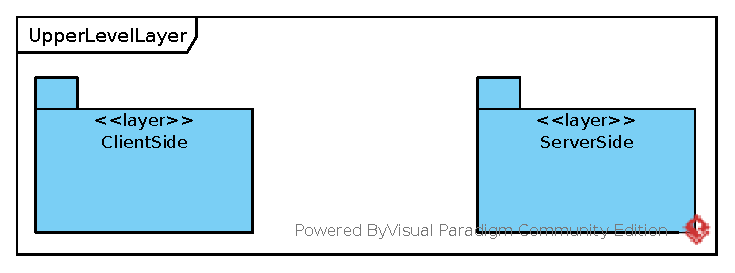
\includegraphics{./images/UpperLevelLayer.eps}
	\end{figure}

	\subsection{Mô tả các lớp kiến trúc mức cao}
	\begin{description}
		\item[Server Side] hỗ trợ nhiều ứng dụng máy chủ khác nhau, bao gồm cả các trang web tĩnh. Máy chủ mạng sẽ biết tới trạng thái tồn tại của máy chủ. Thông thường máy chủ mạng sẽ quản lý máy chủ, tuy nhiên một số trường hợp chương trình ứng dụng sẽ đảm nhiệm một phần trách nhiệm này.
		\item[Client Side]  Lớp này là lớp mà người dùng truy cập ứng dụng. Server Layer tiếp nhận yêu cầu từ client layer thông qua Internet và chuyển các yêu cầu đến các tác nhân thích hợp. Máy chủ sẽ phản hồi lại các tác nhân trở lại  người dùng. Trong trường hợp này, người dùng sẽ chỉ là trình duyệt. 
	\end{description}
	\subsection{Các lớp kiến trúc phụ thuộc}
		\begin{figure}[H]
		\centering
		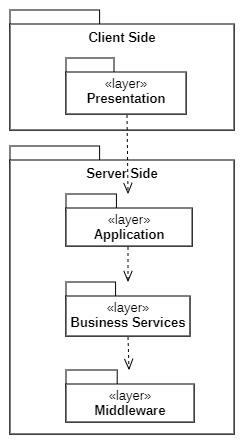
\includegraphics{./images/layer_and_dependencies.png}
	\end{figure}
	\subsection{Mô tả các lớp kiến trúc}
	\begin{description}
		\item[Client Side] Lớp này là lớp mà nơi người dùng truy cập vào ứng dụng. Server layer chấp nhận yêu cầu thông qua kết nối internet từ client layer và chuyển các yêu cầu này đến tác nhân thích hợp. Máy chủ sẽ phản hồi kết quả từ tác nhân trở lại lớp người dùng. Trong trường hợp này, người dùng chỉ đơn giản là một trình duyệt.
		\item[Presentation] Chứa các lớp cho mỗi biểu mẫu mà các tác nhân sử dụng để giao tiếp với Hệ thống.
		\item[Server Side] Server layer hỗ trợ nhiều ứng dụng máy chủ khác nhau, trong đó “ứng dụng” bao gồm cả các trang web tĩnh. Máy chủ mạng sẽ biết trạng thái của máy chủ có tồn tại hay không. Thông thường, các máy chủ thường được quản lý bởi máy chủ mạng, tuy nhiên chương trình ứng dụng có thể đảm nhận một phần trách nhiệm này.
		\item[Application] Chứa các lớp ứng dụng của các phần tử thiết kế cho chức năng xử lý chính của hệ thống.
		\item[Business Services] Chứa các lớp để cung cấp các lớp hệ thống cho mục đích bảo trì.
		\item[Middleware] Cung cấp các tiện ích và nền tảng dịch vụ độc lập.
		
	\end{description}
	\subsection{Các gói và phụ thuộc}
	\subsubsection{Biểu đồ phụ thuộc các gói}
	\begin{figure}[H]
		\centering
		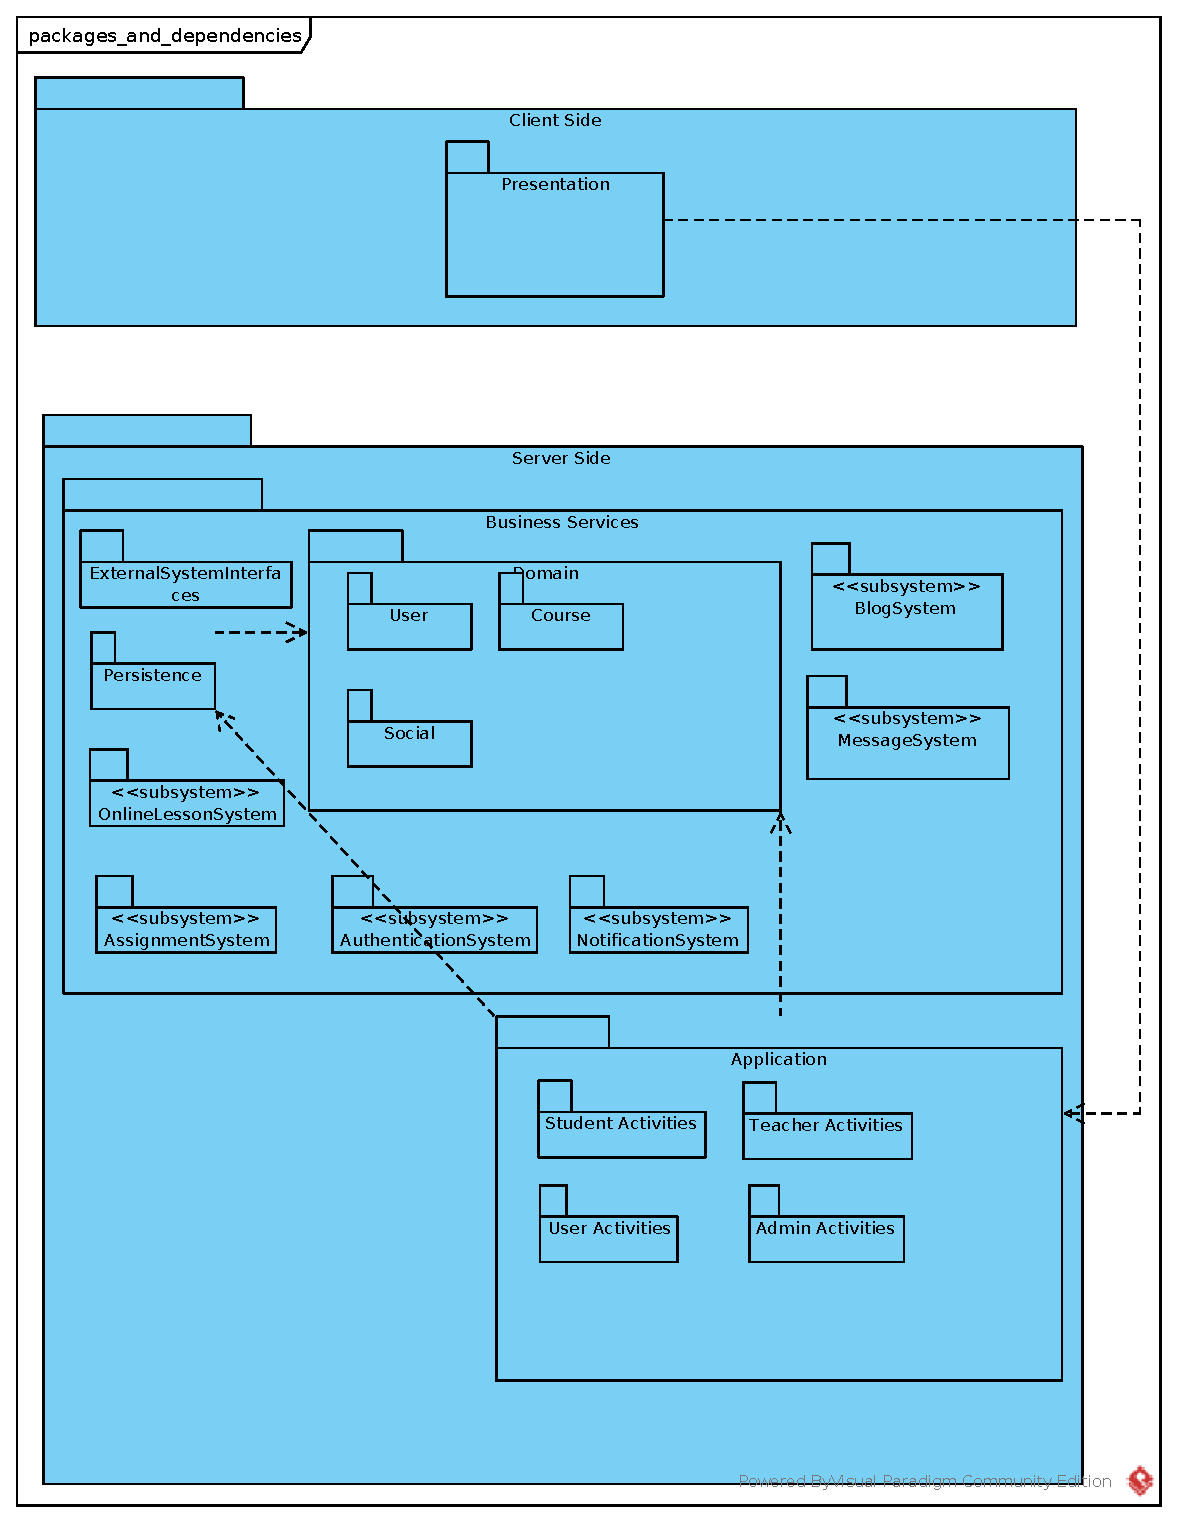
\includegraphics[width=\linewidth]{./images/packages_and_dependencies.eps}
	\end{figure}
	\subsubsection{Mô tả các gói}
	\begin{description}
		\item[Client Side] Là gói mà người dùng sử dụng để tương tác với hệ thống.
		\item[Presentation] Gói chứa các trang giao diện mà người dùng sử dụng.
		\item[Server Side] Gói chứa các lớp thực hiện xử lý các yêu cầu từ Client Side.
		\item[Business Services] Là gói chứa các lớp liên quan đến chức năng thuộc miền nghiệp vụ của hệ thống. Với Hệ thống hỗ trợ học tập và giảng dạy trực tuyến, gói này sẽ chứa các lớp tính năng liên quan đến quản lý khóa học, tổ chức lớp học trực tuyến, nhắn tin, …
		\item[Domain] Gói này chứa các phần tử thiết kế để hỗ trợ về mặt người dùng. Các phần tử bao gồm User (người dùng), Social (xã hội) và Course (khóa học).
		\item[User] Gói chứa phần tử thiết kế liên quan tới xác thực và chỉnh sửa thông tin người dùng.
		\item[Social] Gói chứa phần tử thiết kế liên quan đến tính năng giao tiếp giữa người dùng trên hệ thống: tính năng nhắn tin, đăng blog trên trang cá nhân và thông báo.
		\item[Course] Gói chứa phần tử thiết kế liên quan đến tính năng khóa học: quản lý khóa học, tạo và nộp bài tập, tạo và làm bài kiểm tra, đăng tài liệu và đăng bài trong forum.
		\item[Persistence] Gói chứa các phần tử thiết kế thực hiện tính năng lưu trữ: tạo mới, đọc, cập nhật và xóa.
		\item[Application] Gói chứa các phần tử thiết kế dành riêng cho hệ thống này.
		\item[User Activities] Gói chứa các phần tử thiết kế hỗ trợ chức năng quản lý thông tin cá nhân cho tất cả người dùng.
		\item[Student Activities] Gói chứa các phần tử thiết kế hỗ trợ chức năng cho người dùng học sinh: tham gia khóa học, tham giả buổi học trực tuyến đăng bài trong forum khóa học, gửi bài nộp, làm bài kiểm tra, tải tài liệu lớp học và xem kết quả học tập.
		\item[Teacher Activities] Gói chứa các phần tử thiết kế hỗ trợ chức năng cho người dùng giảng viên, bao gồm tạo buổi học trực tuyến, chia sẻ tài liệu, quản lý khóa học đang dạy, tạo bài tập và tạo bài kiểm tra.
		\item[Admin Activities] Gói chứa các phần tử thiết kế hỗ trợ chức năng cho người dùng quản trị viên, bao gồm quản lý toàn bộ khóa học trên hệ thống và quản lý người dùng.
	\end{description}
\end{document}